\documentclass[a4paper,14pt]{extarticle}

\usepackage[a4paper,top=20mm,bottom=20mm,left=30mm,right=10mm]{geometry}
\usepackage[T1,T2A]{fontenc}
\usepackage[utf8]{inputenc}
\usepackage[russian]{babel}
\usepackage{indentfirst}
\usepackage{titlesec}
\usepackage{graphicx}

\renewcommand{\baselinestretch}{1.3}
\titleformat{\section}{\normalsize\bfseries}{\thesection}{1em}{}
\titleformat{\subsection}{\normalsize\bfseries}{\thesection}{1em}{}
\setlength{\parindent}{12.5mm}

\begin{document}
	
	\newpage\thispagestyle{empty}
	\begin{center}
		\MakeUppercase{
			Министерство науки и высшего образования Российской Федерации\\
			Федеральное государственное бюджетное образовательное учреждение высшего образования\\
			<<Вятский Государственный Университет>>\\
		}
		Институт математики и информационных систем\\
		Факультет автоматики и вычислительной техники\\
		Кафедра электронных вычислительных машин
	\end{center}
	\vfill
	
	\begin{center}
		Отчет по лабораторной работе №8\\
		по дисциплине\\
		<<Информатика>>\\
		<<Разработка последовательных схем (счетчиков)>>
	\end{center}
	\vfill
	
	\noindent
	\begin{tabular}{ll}
		Выполнил студент гр. ИВТб-1301-05-00 \hspace{5mm} &
		\rule[-1mm]{25mm}{0.10mm}\,/Макаров С.А./\\
		
		Руководитель доцент кафедры ЭВМ & \rule[-1mm]{25mm}{0.10mm}\,/Коржавина А.С./\\
	\end{tabular}
	
	\vfill
	\begin{center}
		Киров 2024
	\end{center}
	
	\newpage
	\section*{Цель}
	Цель лабораторной работы: закрепить на практике знания об элементах памяти и последовательных устройствах и получить навыки их реализации.
	
	\section*{Задание}
	\begin{enumerate}
		\item Построить схемы прямого (на +1) и обратного (на -1) 4-разрядных двоичных счетчиков на счетных (T) триггерах. Построить схемы счетчиков в Logisim, проверить их работоспособность.
		
		\item Построить схему прямого счетчика по модулю 10, то есть считающего в прямом направлении от 0 до 9 на счетных (T) триггерах. Построить схему счетчика в Logisim, проверить его работоспособность.
		
		\item Построить схему прямого счетчика по произвольному модулю N, то есть считающего в прямом направлении от 0 до N-1 на счетных (T) триггерах. Построить схему счетчика в Logisim, проверить его работоспособность.
		
		\item Построить схему прямого счетчика по произвольному модулю N, то есть считающего в прямом направлении от 0 до N-1 на D триггерах. Построить схему счетчика в Logisim, проверить его работоспособность.
		
		\item Построить схему прямого счетчика на +3. Счетчик увеличивает значение на +3, то есть счет идет 0 3 6 9 12 15 0 и т.д. на T триггерах. Построить схему счетчика в Logisim, проверить его работоспособность.
		
		\item Построить схему прямого счетчика на +5. Счетчик увеличивает значение на +5, то есть счет идет 0 5 10 15 20 25 30 0 и т.д. на T триггерах. Построить схему счетчика в Logisim, проверить его работоспособность.
		
	\end{enumerate}
	
	\newpage
	\section*{Решение}
	\subsection*{Задание 1}
	Комбинационная схема прямого 4-разрядного счетчика представлена на рисунке 1, схема обратного счетчика представлена на рисунке 2.
	
	\begin{figure}[h]
		\centering
		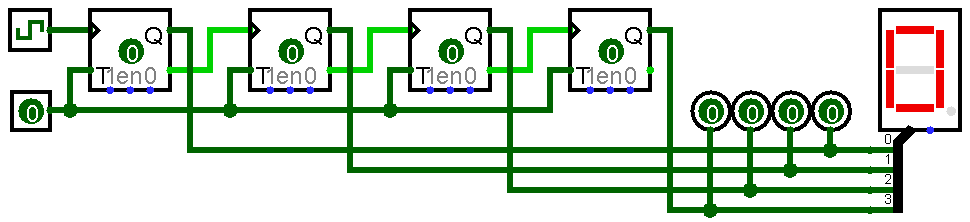
\includegraphics[width=0.8\linewidth]{images/s-1-1}
	\end{figure}
	\begin{center}
		Рисунок 1 – Прямой 4-разрядный счетчик
	\end{center}
	
	\begin{figure}[h]
		\centering
		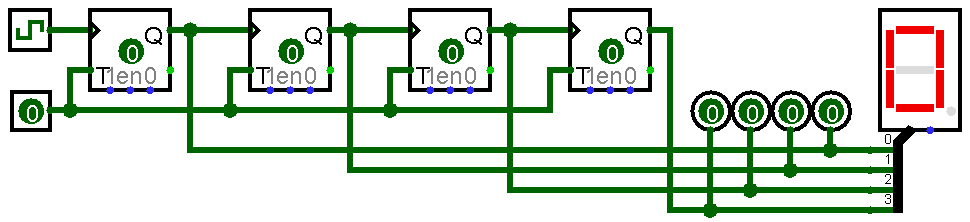
\includegraphics[width=0.8\linewidth]{images/s-1-2}
	\end{figure}
	\begin{center}
		Рисунок 2 – Обратный 4-разрядный счетчик
	\end{center}
	
	\subsection*{Задание 2}
	Комбинационная схема прямого счетчика по модулю 10 представлена на рисунке 3.
	
	\begin{figure}[h]
		\centering
		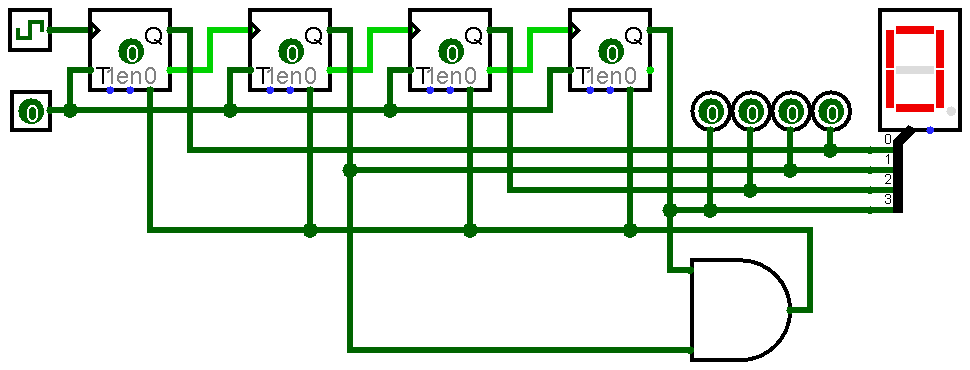
\includegraphics[width=0.8\linewidth]{images/s-2}
	\end{figure}
	\begin{center}
		Рисунок 3 – Прямой счетчик по модулю 10
	\end{center}
	
	\subsection*{Задание 3}
	Комбинационная схема сброса счетчика представлена на рисунке 4. Схема прямого счетчика по произвольному модулю представлена на рисунке 5.
	
	\begin{figure}[h]
		\centering
		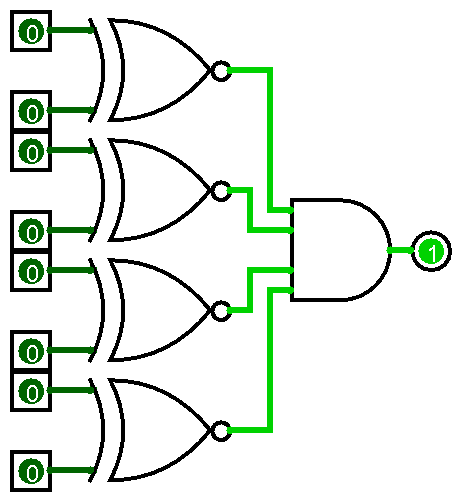
\includegraphics[width=0.4\linewidth]{images/s-3-1}
	\end{figure}
	\begin{center}
		Рисунок 4 – Схема сброса счетчика
	\end{center}
	
	\begin{figure}[h]
		\centering
		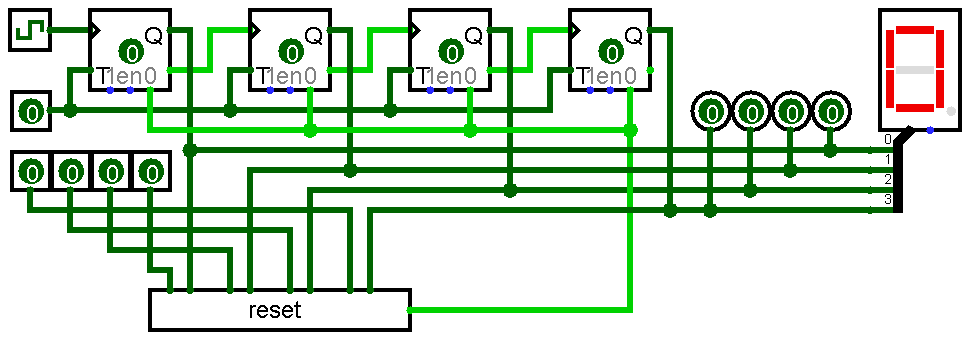
\includegraphics[width=0.8\linewidth]{images/s-3-2}
	\end{figure}
	\begin{center}
		Рисунок 5 – Прямой счетчик по произвольному модулю
	\end{center}
	
	\pagebreak
	\subsection*{Задание 4}
	Комбинационная схема прямого счетчика по произвольному модулю на D-триггерах представлена на рисунке 6
	
	\begin{figure}[h]
		\centering
		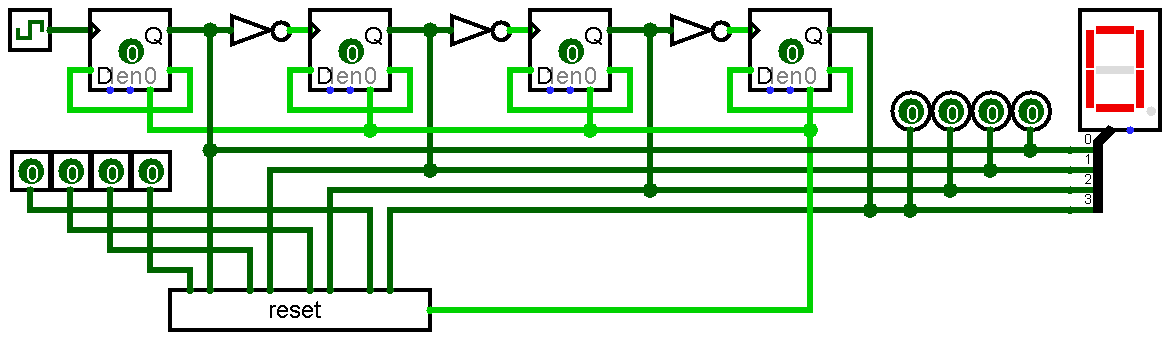
\includegraphics[width=0.8\linewidth]{images/s-4}
	\end{figure}
	\begin{center}
		Рисунок 6 – Прямой счетчик по произвольному модулю на D-триггерах
	\end{center}
	
	\subsection*{Задание 5}
	Комбинационная схема прямого счетчика на +3, построенного на T-триггерах, представлена на рисунке 7.
	
	\begin{figure}[h]
		\centering
		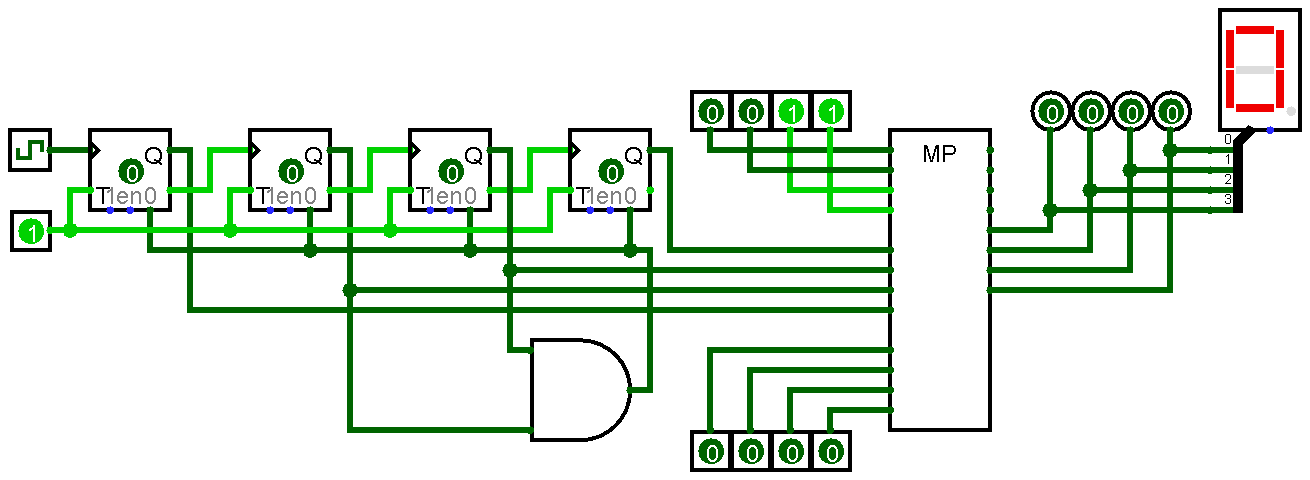
\includegraphics[width=0.8\linewidth]{images/s-5}
	\end{figure}
	\begin{center}
		Рисунок 7 – Прямой счетчик на +3
	\end{center}
	
	\pagebreak
	\subsection*{Задание 6}
	Комбинационная схема прямого счетчика на +5, построенного на T-триггерах, представлена на рисунке 8.
	
	\begin{figure}[h]
		\centering
		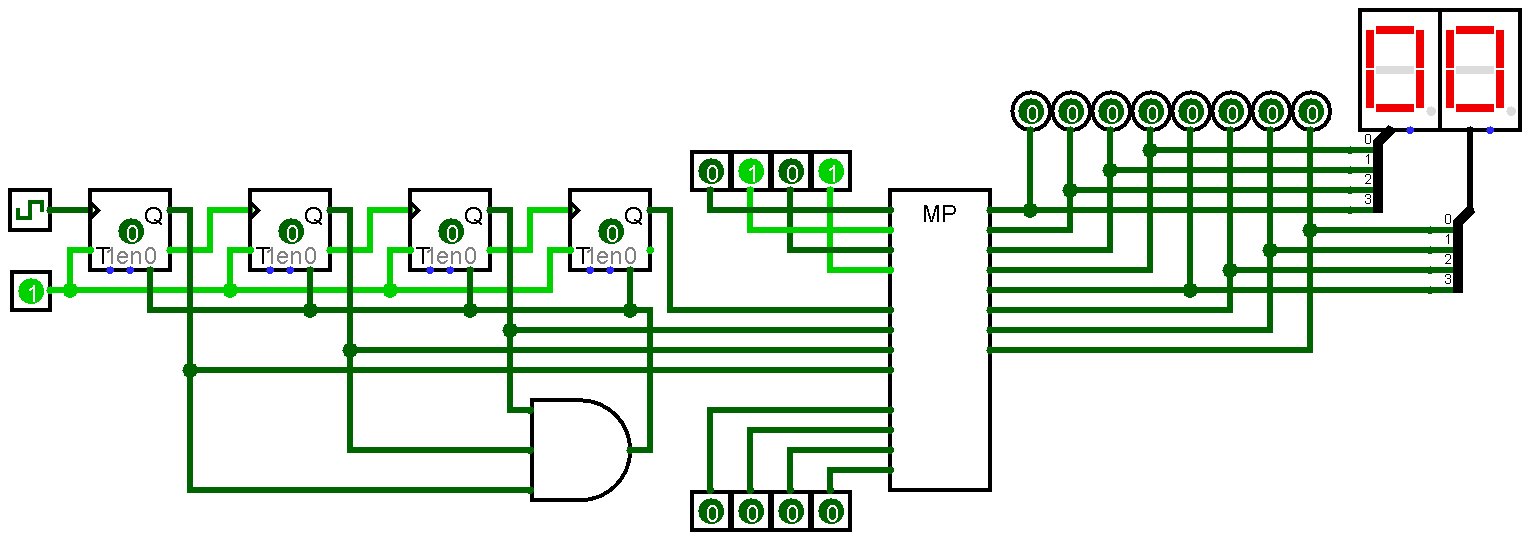
\includegraphics[width=0.8\linewidth]{images/s-6}
	\end{figure}
	\begin{center}
		Рисунок 8 – Прямой счетчик на +5
	\end{center}
	
	\section*{Вывод}
	В ходе лабораторной работы были закреплены на практике знания об элементах памяти и последовательных устройств. Были реализованы схемы прямого (на +1) и обратного (на -1) счетчика на T-триггерах, схема прямого счетчика по модулю 10, схема прямого счетчика по произвольному модулю на T и D триггерах, схемы прямых счетчиков на +3 и +5.
	
\end{document}